
Como este código es muy complicado de paralelizar, limitaremos el problema a dos procesadores, para simplificar el paso de datos.

Antes de comenzar a ordenar los datos es necesario calcular el máximo de todos los elementos, ya que influye en el número de ejecuciones del algoritmo, por lo tanto, es necesario que todos los procesos conozcan este dato. Todos los procesos tienen que ejecutar el mismo número de iteraciones, aunque puede que alguno no necesite hacer tantas, para sincronizar el paso de datos final, con el array ordenado.
Esto se hace con MPI\_Allreduce, que realiza la operación indicada (MPI\_MAX en este caso) sobre el dato indicado (m) y comparte el resultado con \textbf{todos} los procesos.
\begin{lstlisting}[frame=single]
	m = maximo(a, n);
	MPI_Allreduce(&m, &m, 1, MPI_INT, MPI_MAX, MPI_COMM_WORLD);
\end{lstlisting}

El bucket se recalcula en cada iteración, por lo que también es necesario compartirlo en cada iteración. Radixsort ordena en función de la suma acumulada del bucket.

El trabajo de realizar la suma acumulativa lo hace el proceso 1 y le manda el resultado al 0. Es necesario hacerlo de este modo, ya que se utiliza el bucket acumulado para calcular las posiciones destino de los elementos del array a, ordenándolo en cada iteración.

El cálculo de las posiciones destino se hace desde el final al principio del array a ordenar (así lo requiere el algoritmo). Además, se resta el bucket para obtener la posición destino por lo que, al paralelizarlo, es necesario secuencializar esta parte de los procesos, de modo que sigan el mismo orden que el secuencial. Para ello, los elementos se envían en orden \emph{inverso} de procesos (desde el proceso n al $n-1$, del $n-1$ al $n-2$, ...).

% a_intercambio
Es raro que, al dividir los datos a ordenar entre dos procesos, coincida que los datos del proceso 0 pertenezcan a la primera mitad del array a ordenar y los de proceso 1 a la segunda. Es decir, se va a tener que enviar algún dato de \texttt{P0} a \texttt{P1}. Para esto, se van almacenando los datos a intercambiar en un \emph{array de intercambio} y, al final de cada iteración, los procesos intercambian sus \texttt{a\_intercambio} y guardan los datos recibidos.

\begin{lstlisting}[frame=single]
// El P0 se queda esperando por los datos del P1
if(myrank==0){
	MPI_Recv(a_intercambio, elemTot, MPI_INT, 1, 3, MPI_COMM_WORLD, &status);
	MPI_Recv(&bucket[0], 10, MPI_INT, 1, 4, MPI_COMM_WORLD, &status);
	for(i=0;i<elemTot;i++){
		if(a_intercambio[i]!=-1){
			// Se adapta la posicion del otro proceso
			pos_envio = i % n;
			b[pos_envio] = a_intercambio[i];
		}
	}
	inicializar_array(&a_intercambio[0], elemTot, -1);
}
\end{lstlisting}

Este array tiene las dimensiones del array total. Se ha decidido implementarlo así, aunque pueda suponer una mayor carga de memoria, porque los procesos no siempre van a querer enviar datos en el mismo instante, lo que supondría que los procesos se quedaran esperando mútuamente y repercutiría mucho sobre el tiempo de ejecución.

\texttt{a\_intercambio} tiene las dimensiones del array total porque los elementos a intercambiar ya se guardan en la posición destino del otro proceso. De este modo, al guardar los datos en \texttt{a\_intercambio}, cada proceso tiene que adaptar la posición en la que se guarda al otro proceso.


Cuando el \texttt{P1} acaba una iteración, envía el bucket y el a\_intercambio al \texttt{P0} y se queda esperando por el a\_intercambio de \texttt{P0}.
\begin{lstlisting}[frame=single]
if(myrank==1){
	MPI_Send(a_intercambio, elemTot, MPI_INT, 0, 3, MPI_COMM_WORLD);
	MPI_Send(&bucket[0], 10, MPI_INT, 0, 4, MPI_COMM_WORLD);
	MPI_Recv(a_intercambio, elemTot, MPI_INT, 0, 5, MPI_COMM_WORLD, &status);

	for(i=0;i<n;i++){
		if(a_intercambio[i]!=-1){
			b[i] = a_intercambio[i];
		}
	}
	inicializar_array(&a_intercambio[0], elemTot, -1);
}
\end{lstlisting}

Al final de cada iteración del bucle, cada proceso recibe el \texttt{a\_intercambio} del otro proceso, lo guarda en su array \texttt{b} local y, finalmente, lo almacena en \texttt{a}.


Como se puede ver en la gráfica de la figura \ref{grafica_mpi}, no se consiguen mejoras en este ejemplo usando \texttt{MPI} con dos procesadores. Esto se debe al gran paso de datos entre procesadores, la secuencialización de un trozo del código y el hecho de sólo usar dos procesadores. Además, cuando mayor sea el máximo elemento del array a ordenar, más iteraciones tiene que hacer el algoritmo, mayor paso de datos en la paralelización \texttt{MPI} y mayor ineficiencia.

\begin{figure}[h]
	\centering
	\lstinputlisting{./res/tabla_mpi}
	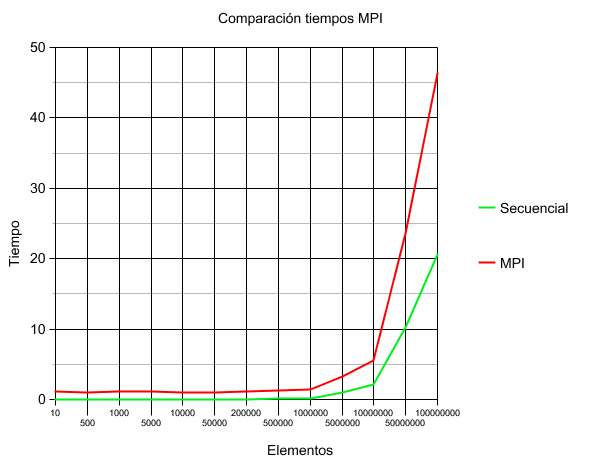
\includegraphics[width=1\textwidth]{./res/grafica_mpi}
	\label{grafica_mpi}
\end{figure}